\documentclass[a4paper,10pt]{report}
\usepackage[utf8]{inputenc}
\usepackage{mathtools}
\usepackage{algorithm}
\usepackage{algorithmic}
\renewcommand{\algorithmicrequire}{\textbf{Input: }}
\renewcommand{\algorithmicensure}{\textbf{Output: }}

\begin{document}

\section*{Modularidade}

Modularidade de uma partição para grafos com pesos nas arestas:

\begin{equation}
Q = \frac{1}{2m} \sum_{i,j} [ A_{ij} - \frac{k_i k_j}{2m} ] \delta(c_i ,c_j)
\label{eq:MN}
\end{equation}


\begin{itemize}
	\item $A_{ij}$ é o peso da aresta entre $i$ e $j$.
	\item $k_i = \sum_j A_{ij}$ é a soma do peso de todas as arestas de $i$, com o mesmo significado para $k_j$.
	\item $c_i$ é a comunidade de $i$, com o mesmo significado para $c_j$.
	\item $\delta(c_i,c_j)$ é a igualdade entre $c_i$ e $c_j$ ( as duas vértices serem da mesma comunidade).
	\item $m = \frac{1}{2}\sum_{ij} A_{ij}$ é a soma do peso de todos as arestas %metade porque consideram que 
%o peso das arestas será calculado duas vezes, por cada vértice. Logo é necessário dividir.
\end{itemize}

A modularidade mede a densidade das arestas dentro das comunidades em comparação com aquelas entre comunidades e é usada para saber a qualidade da partição de um grafo em comunidades criadas por um método. 


\section*{Louvain Method}
Algoritmos existentes para cálculo de modularidade em grafos são muito pouco eficientes para grafos de larga escala e é também necessário detetar as comunidades dentro de comunidades (sub-comunidades).

As suas duas fases são:

\paragraph{Primeira}
Todos os vértices têm uma comunidade diferente, sendo que existem N comunidades onde N é o número de vértices.
Para cada nó é visto os seus adjacentes e calculado o ganho de modularidade que existiria se o nó fosse adicionado à comunidade do vizinho. Sendo adicionado à comunidade do vizinho com o maior ganho não negativo. Esta fase continua até já não existir ganhos (modularidade máxima).
O ganho obtido movendo um nó isolado $i$ para uma comunidade $C$ é calculado através da equação:


\begin{equation}
\label{eq:GND}
 \Delta Q  =  [\frac{\sum_{in} + k_{i,in}}{2m} - (\frac{\sum_{tot} +k_i}{2m})^2] - [\frac{\sum_{in}}{2m} - (\frac{\sum_{tot}}{2m})^2 - (\frac{k_i}{2m})^2] 
\end{equation}

\begin{itemize}
	\item $\sum_{in}$ é a soma do peso de todas as arestas dentro de $C$ (vão de um vértice em C para outro)
	\item $\sum_{tot}$ é a soma do peso de todas as arestas dos vértices de $C$. %( inclui Ein ou é aqueles que vão de outros vértices para os da comunidade C?)
	\item $K_i$ é a soma do peso de todas as arestas de $i$. %(incidentes...)
	\item $K_{i,in}$ é a soma do peso de todas as arestas de $i$ para vértices de $C$.
	\item $m$ é soma de do peso total do grafo.
\end{itemize}

\paragraph{Segunda}
É criado um novo grafo cujo vértices sejam as comunidades anteriormente encontradas e o peso da aresta entre duas comunidades é calculado somando o peso de todas as arestas entre estas. É depois aplicada novamente a 1ª fase a este novo grafo.
Estas duas fases são nomeadas 'passos' e continuam até ser encontrada a modularidade máxima.


É assim apresentado o seguinte algoritmo onde \verb|i| representa um vértice, \verb|comm| uma comunidade, \verb|comm[i]| a comunidade de \verb|i|, \verb|tot[comm]| representa $E_{tot}$ para a comunidade \verb|comm| e \verb|m2| é $2m$.
\begin{algorithm}
\caption{Primeiro passo}
\label{alg:LMPS}

	\algorithmicrequire{Grafo G}
	\begin{enumerate}
		\item Para todos os vértices $i$ em $G$ $comm[i] \gets i$
		\label{SS1}
		\item Remover $i$ da sua comunidade atual $comm[i]$
		\item Para todos os vizinhos $j$ de $i$ $comm \gets comm[j]$ e computar o ganho conseguido em mover $i$ para $comm$ $curr\_gain \gets computeGain(i,comm,m2)$
		\item Inserir $i$ na comunidade com o maior ganho atualizando o $tot[comm]$ de acordo.
		\item Se algum $i$ foi movido para uma comunidade diferente então voltar para ~\ref{SS1}.
	\end{enumerate}
\end{algorithm}


Neste algoritmo $computeGain$ calcula o ganho usando a equação referida em cima.

\begin{algorithm}
\caption{Segundo passo}
	\begin{enumerate}
		\item Se ocorreu alguma mudança de comunidade no passo anterior
		\item Passar todos os vértices $i$ na mesma comunidade para uma só comunidade
		\item O peso das arestas entre duas comunidades passa a ser a soma do peso das arestas dos nós entre duas comunidades e as arestas para a mesma comunidade passam a ser nós circulares
		\item Voltar a executar o algoritmo \ref{alg:LMPS} com o novo grafo formado.
	\end{enumerate}
\end{algorithm}

O exemplo seguinte tem um total de 25 arestas, sendo que o seu \verb|m2| será 50:
\begin{figure}
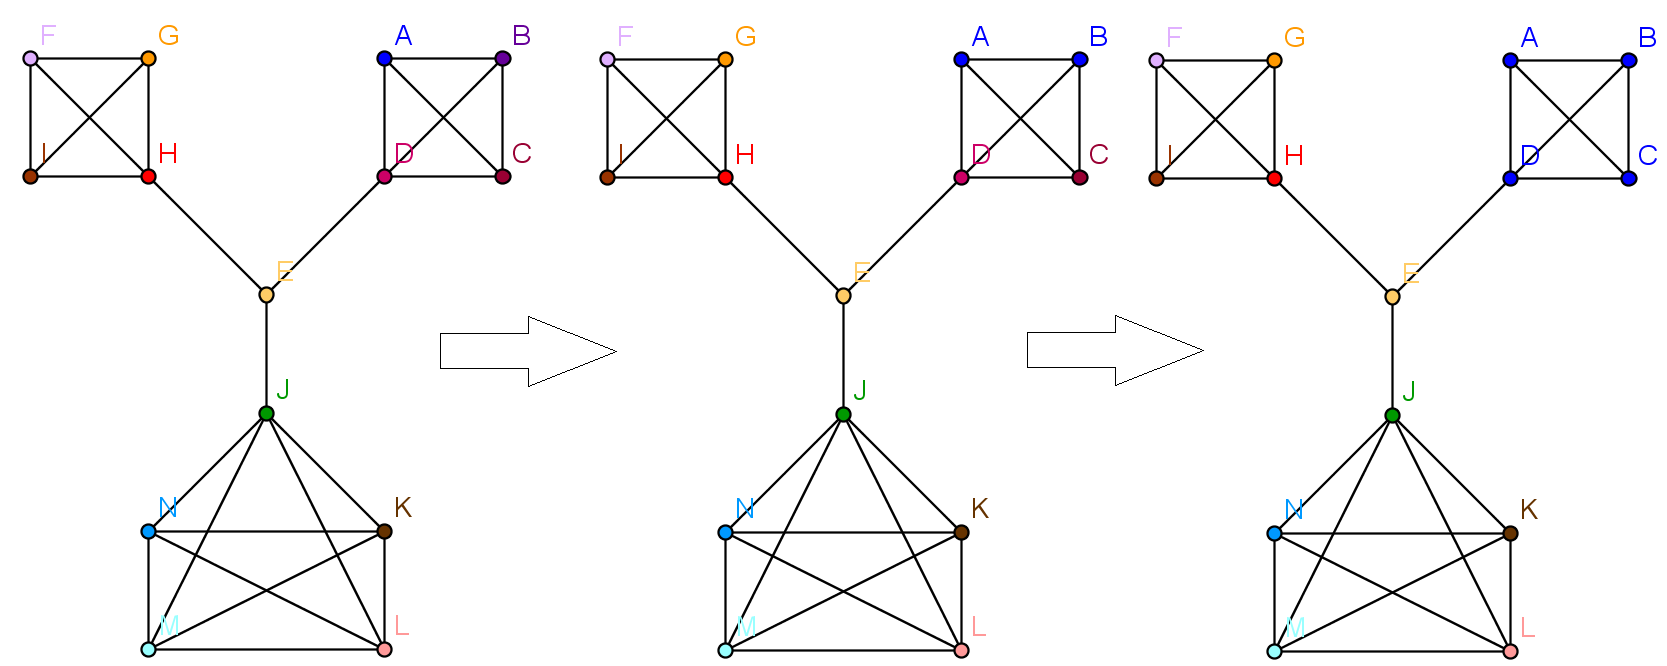
\includegraphics[width=90mm]{graphf1}
\caption{Todas as vértices começam por por a sua comunidade igual ao seu id. De seguida, são removidos da comunidade atual e é calculado o ganho em inserir-los na comunidade de uns dos vizinhos, sendo posto na comunidade com o maior ganho.}
\end{figure}
\begin{figure}
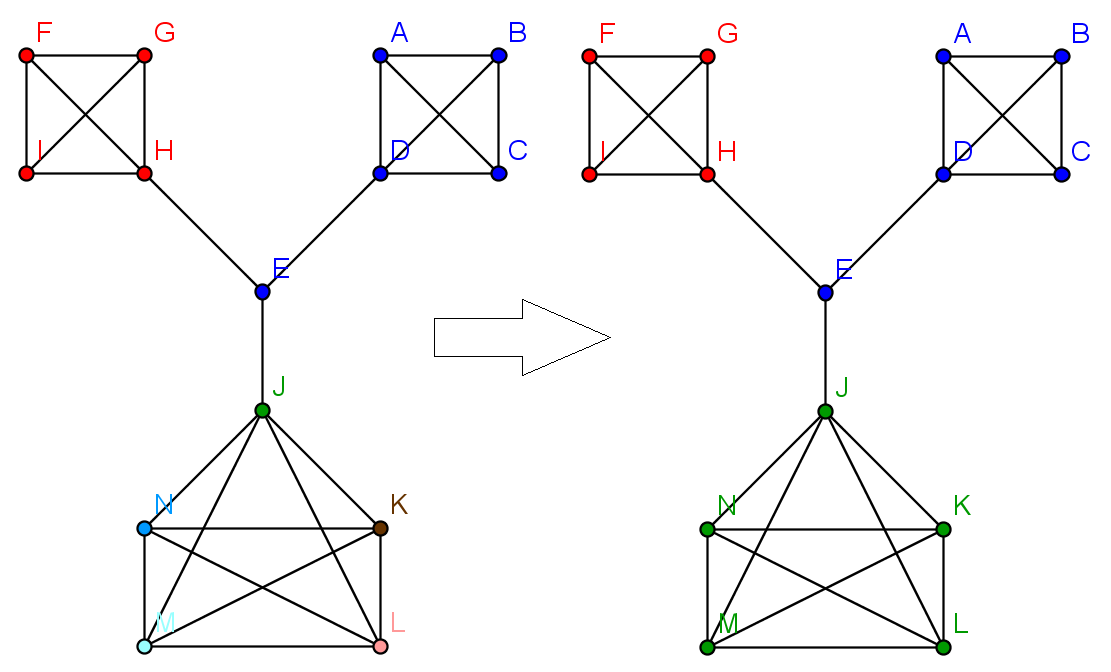
\includegraphics[width=90mm]{graphf2}
\caption{Este processo continua até nenhuma vértice mover de comunidade.}
\end{figure}
\begin{figure}
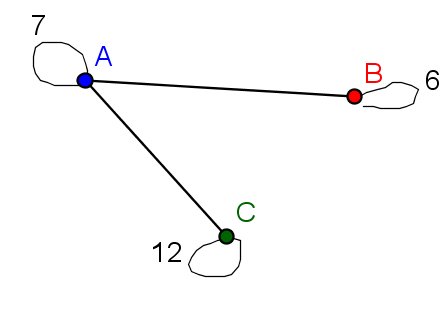
\includegraphics[width=90mm]{graphf3}
\caption{No segundo passo as comunidades existentes passam a só um grafo e as arestas dentro da comunidade passam a ser uma única circular. É depois executado o primeiro passo mas neste exemplo já não ocorrem alterações.}
\end{figure}


\newpage
\section*{Louvain Method Distribuído}
O método apresentado anteriormente pode ser usado para grafos de larga escala, mas o tamanho do grafo está limitado pela memória disponível na máquina.

É possível resolver a equação \ref{eq:GND} e obter a equação:
\begin{equation}
	\Delta Q  =  K_{i,in} - \frac{\sum_{tot} K_i}{2m}
\label{eq:GD}
\end{equation}


Esta nova equação depende de menos variáveis e, visto que $K_{i,in}$ e $K_i$ são referentes a um único vértice, leva a que seja necessário trocar menos informação entre os vários vértices na versão distribuída deste método.
\end{document}